% In your .tex file
% !TEX program = xelatex

\documentclass{article} % For LaTeX2e
\usepackage{nips15submit_e,times}

\usepackage{hyperref}
\usepackage{url}
\usepackage[toc,page]{appendix}

%citation
\usepackage[backend=bibtex]{biblatex}
\bibliography{openbrain}
%

% tikz and associated macros
\usepackage{tikz}

\usetikzlibrary{decorations.pathmorphing}
\tikzset{snake it/.style={decorate, decoration=snake}}
%

% math
\usepackage{amsthm}
\usepackage{amsmath}
\usepackage{amssymb}
\usepackage{mathabx}
\newcommand{\BlackBox}{\rule{1.5ex}{1.5ex}}  % end of proof
\newtheorem{example}{Example} 
\newtheorem{theorem}{Theorem}
\newtheorem{lemma}[theorem]{Lemma} 
\newtheorem{proposition}[theorem]{Proposition} 
\newtheorem{remark}[theorem]{Remark}
\newtheorem{corollary}[theorem]{Corollary}
\newtheorem{definition}[theorem]{Definition}
\newtheorem{conjecture}[theorem]{Conjecture}
\newtheorem{axiom}[theorem]{Axiom}

\numberwithin{equation}{subsection}
\numberwithin{theorem}{subsection}

\DeclareSymbolFont{cmlargesymbols}{OMX}{cmex}{m}{n}
\let\sumop\relax
\DeclareMathSymbol{\sumop}{\mathop}{cmlargesymbols}{"50}

%

%% todo[inline] NOTES. To remove for camera ready version.
\usepackage{todonotes}
\usepackage{regexpatch}
%end to notes

\title{OpenBrain: Massively Asynchronous Neurocomputation}


\author{
William H.~Guss \\
Machine Learning at Berkeley\\
2650 Durant Ave, Berkeley CA, 94720 \\
\texttt{wguss@ml.berkeley.edu} \\
\And
Mike Zhong \\
Machine Learning at Berkeley \\
Berkeley CA, 94720 \\
\texttt{lol@gmail.com} \\
\And
Phillip Kuznetsov \\
Machine Learning at Berkeley \\
Berkeley CA, 94720 \\
\texttt{philkuz@ml.berkeley.edu} \\
\And
Jacky Liang \\
Machine Learning at Berkeley \\
Berkeley CA, 94720 \\
\texttt{jackyliang@berkeley.edu} \\
\And
Instert yourself \\
Machine Learning at Berkeley \\
Address \\
\texttt{email} \\
\And
We can add footnotes clarifying \\
Machine Learning at Berkeley \\
Address \\
\texttt{email} \\
\And
equal contributions to the work \\
(if needed)\\
Machine Learning at Berkeley \\
Address \\
\texttt{email} 
}


\nipsfinalcopy % Uncomment for camera-ready version

\begin{document}


\maketitle

\begin{abstract}
	In this paper we introduce a new framework and philosophy for recurrent neurocomputation. By requiring that all neurons act asynchrynously and independently, we introduce a new metric for evaluating the universal intelligence of continuous time agents. We proved representation and universal approximation results in this context which lead to a set of learning rules in the spirt of John Conway's game of life. Finally evaluate this framework against different intelligent agent algorithms by implementing an approximate universal intelligence measure for agents embedded in turing computable environments in Minecraft, BF, and a variety of other reference machines. 
\end{abstract}


\listoftodos
%!TEX root = main.tex
\section{Introduction}
\emph{Note:} 
We need to motivate substantially the proposal of a drastically different framework of neurocomputation. This motivation should be given according to the latest neuroscience, and a general problem in the field.

\todo{Argue against 
the current state of ML's approach to the problem of AGI
by surveying field.}
\subsection{Intelligence as an Emergence Phenomenon}
\todo{Establish Conwaynian philosophy on emergent neurocomputation.}
\todo{Motivate asynchrynous neurocomputation.}

%!TEX root = main.tex
\section{Asynchronous Neurocomputation}
\emph{Note:} This section will essentially lay out our model minus learning rules. This means we must give theoretical, biological justifications for the algorithm.

%!TEX root = main.tex
\subsection{The Core Framework}
%!TEX root = ../main.tex
\subsection{Continuous Time Universal Intelligence Measure}

In alignment with the philosophy which predicates OpenBrain, we wish to extend the evaluation of our algorithm well beyond its performance in supervised learning tasks; that is, what can be said about the intelligence of OpenBrain as an agent in an environment? A metric more condusive to implementing general intelligence is needed. The answer will motivate an important discussion of representation theory annd learning rules.
\subsection{Universal Intelligence}
A well established\cite{legg2008machine, mnih2015human, rathmanner2011philosophical}  machine intelligence measure is the Universal Intelligence Measure proposed by Legg and Hutter \cite{legg2007universal}. Drawing from a large amount of disparate literature on the subject they develop a consise definition of the intelligence of an \emph{agent} in an \emph{environment}. 
\todo[inline]{The following exposition may be unnecessary, and we should consider just stating the result of Legg and Hutter.}

Environment-agent interaction is defined with respect to an observation space, $\mathcal{O}$, and an action space, $\mathcal{A}$, both of which consist of abstract symbols. The perception space, $\mathcal{P} \subset \mathcal{O} \times \mathbb{R}$, is the combination of observations and rewards.
\begin{definition}
	An \textbf{environment} $\mu$ is a probability measure, specifically defining
	\begin{equation}
			\mu(o_kr_k | o_1r_1a_1 \dots o_{k-1}r_{k-1}a_{k-1}),
	\end{equation}
	the probability of observing $o_kr_k \in \mathcal{P}$ given a history, a string $o_1\dots a_{k-1} \in \bigtimes_{i=1}^k \mathcal{P} \times \mathcal{A}.$
\end{definition}

In the same light the agent definition is given.
\begin{definition}
	An \textbf{agent} $\pi$ is a probability measure, giving
	\begin{equation}
		\pi(a_k | o_1r_1a_1 \dots a_{k-1}o_kr_k)
	\end{equation}
	the probability of the possible action $a_k$ being enacted by $\pi$ being the environment-agent interaction history.
\end{definition}
\todo[inline]{Include agent environment interaction picture? Would this section be clear given that the reader has explored \cite{legg2007universal}?}

Having defined the basic framework, \cite{legg2007universal} gives a definition for Universal Intelligence. Let $E$ be the space of all turing complete reward environments, and $K: E \to  \mathbb{R}$ be the Kolmogorov complexity of an environment. This complexity is calculated with respect to the length of the string with which a reference machine $\mathcal{U}$ generates the environment.
\begin{definition} \label{uim}
	If $\pi$ is an agent then we say that the \textbf{universal intelligence} of $\pi$ is
	\begin{equation} \label{eq:uim}
		\Upsilon(\pi) = \sumop_{\mu \in E}2^{-K(\mu)}V_\mu^\pi
	\end{equation}
	where $V_\mu^\pi$ is the expected reward of the agent in $\mu$,
	\begin{equation} \label{eq:exprewarduim}
		V_\mu^\pi = \mathbb{E}\left(\sumop_{i=1}^\infty r_i\right) \leq 1.
	\end{equation}
\end{definition}

The definition is satisfactory for agents which act synchronously with their environments; that is, the environment waits for the agent to act before giving a new observation. Therefore in Hutter's sense, the framework of \cite{legg2007universal} describes an agent $\pi$ embedded in $\mu$.

Despite this, the environments which we normally consider an intelligent agent to 'act well' in are often chaotic and operate with noise which is temporally independent from the agent-environment interaction itself. \todo{Why!?} For example, a real time game does not wait for a player to press a key, and yet the player still receives perceptual information. The intelligence measure proposed fails to encompass agent-environment interactions where the agent has some delay in acting as the environment continues; modeling such delays as $a_k = \emptyset$ is no more enlightening.

In order to integrate OpenBrain with this framework, we will propose a continuous time universal intelligence measure.

\subsection{Continuous Time Intelligence}

To make a continuous time intelligence measure which is compatible with agents who act instantaneously within an environment, we will define a completed perception space.

Since different agents 

\begin{definition}
	Given an environment $\mu$ with an associated 
	perception space $\mathcal{P}$ we define the
	\textbf{completion} $\tilde{\mathcal{P}}$ with respect to the admissible sequences of observations in $\mu$; that is,
	\begin{equation}
		\tilde{\mathcal{P}} = \bigsqcup_{k=1}^\infty \mathcal{P}^k.
	\end{equation}
\end{definition}


Pre med = jessica $^2q$
\begin{centering}

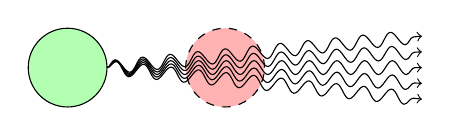
\begin{tikzpicture}
	\draw[style=dashed, fill=red!30] (2,.5) circle (0.5);
	\draw[fill=green!30] (0,0.5) circle(0.5);
	\path[draw, ->, snake it] (0.5,0.5) -- (4.5,.5) ;
	\path[draw, ->, snake it] (0.5,0.5) -- (4.5,.9) ;
	\path[draw, ->, snake it] (0.5,0.5) -- (4.5,.7) ;
	\path[draw, ->, snake it] (0.5,0.5) -- (4.5,.3) ;
	\path[draw, ->, snake it] (0.5,0.5) -- (4.5,.1) ;
\end{tikzpicture} 

\end{centering}
%!TEX root = main.tex
\subsection{Universal Approximation}
\subsection{(optional) Multiprocess Turing Completeness}
If we decide to go down this route, we'll add it's own \TeX file.
%!TEX root = main.tex
\section{Conwaynian Learning Rules}


\section{Experimentation}
\subsection{Implementation}
\subsection{Results}
\section{Conclusion}
\subsection{Future Work}

\printbibliography

\begin{appendices}
\section{Universal Intelligence Definitions}
\end{appendices}

\end{document}